%---------------DOCUMENT SETTINGS------------------------------------
%\documentclass[headheight=30pt]{scrartcl}
\documentclass{article}

\usepackage[utf8]{inputenc} % utf8x durch utf8 ersetzt wegen biblatex
\usepackage[T1]{fontenc}
\usepackage{amsmath,amssymb,amstext,amsfonts}
\usepackage[ngerman]{babel}
\usepackage{csquotes}
\usepackage{pdfpages} %zum importieren des Deckblattes
\usepackage{geometry}
\usepackage[headsepline]{scrlayer-scrpage}
\usepackage{lastpage}
\usepackage[style=numeric]{biblatex} %Literaturverwaltung
\usepackage{tabularx} %für die Legende im Gruundlagen Oszi Bild
\usepackage{tabulary}
\usepackage{float}
\usepackage{textcomp}
\usepackage{gensymb}
\usepackage{physics}
\usepackage{stmaryrd}
\usepackage{graphicx}
\usepackage[export]{adjustbox}
\usepackage{a4wide}
\usepackage{siunitx}
\usepackage{hyperref}
\usepackage{multicol}
\usepackage{makecell}
\usepackage{enumitem}
\usepackage{subcaption}


\geometry{      %holt mehr aus einer A4 Seite raus
    a4paper,
    total={170mm,257mm},
    left=20mm,
    top=25mm,
   }
\graphicspath{ {./graphics/} }  %pfad für bilder
\hypersetup{colorlinks=false}
\addbibresource{literatur.bib} %Literatur-Resourcen\s
%\setlength{\headheight}{0.0pt} % macht zwar headheight warnings aber dafür nutz latex die seitengröße besser aus.
\pagestyle{scrheadings}
\newcommand{\subf}[2]{
    {
        \begin{tabular}[c]{@{}c@{}}
            {\setlength{\extrarowheight}{100pt} #1 }\\#2
        \end{tabular}
    }
}
\newcommand{\allc}{\multicolumn{1}{c|}{-}}
\newcommand{\monofig}[4]{
    
    \begin{figure}[H]
    \centering
    \includegraphics[#1]{#2}
    \caption{
        #3
    }
    \label{#4}
    \end{figure}
    
}
\newcommand{\polyfig}[6]{
    \begin{figure}[H]
        \centering
        \begin{minipage}[b]{0.45\textwidth}
            \centering
            \includegraphics[width=\textwidth]{#1}
            \caption{#2}
            \label{#3}
        \end{minipage}
        \begin{minipage}[b]{0.45\textwidth}
            \centering
            \includegraphics[width=\textwidth]{#4}
            \caption{#5}
            \label{#6}
        \end{minipage}
    \end{figure}
}
\newcommand{\polyfigacc}[8]{
    \begin{figure}[H]
        \centering
        \begin{minipage}[b]{#1}
            \centering
            \includegraphics[width=\textwidth]{#2}
            \caption{#3}
            \label{#4}
        \end{minipage}
        \begin{minipage}[b]{#5}
            \centering
            \includegraphics[width=\textwidth]{#6}
            \caption{#7}
            \label{#8}
        \end{minipage}
    \end{figure}
}
\newcommand{\trifig}[9]{
    \begin{figure}[H]
        \centering
        \begin{minipage}[b]{0.32\textwidth}
            \centering
            \includegraphics[width=\textwidth]{#1}
            \caption{#2}
            \label{#3}
        \end{minipage}
        \begin{minipage}[b]{0.32\textwidth}
            \centering
            \includegraphics[width=\textwidth]{#4}
            \caption{#5}
            \label{#6}
        \end{minipage}
        \begin{minipage}[b]{0.32\textwidth}
            \centering
            \includegraphics[width=\textwidth]{#7}
            \caption{#8}
            \label{#9}
        \end{minipage}
        \caption{#10}
        \label{#11}
    \end{figure}
}
\newcommand{\trifigcom}[8]{
    \begin{figure}[H]
        \centering
        \begin{subfigure}[b]{0.32\textwidth}
            \centering
            \includegraphics[width=\textwidth]{#1}
            \caption{}
            \label{#2}
        \end{subfigure}
        \begin{subfigure}[b]{0.32\textwidth}
            \centering
            \includegraphics[width=\textwidth]{#3}
            \caption{}
            \label{#4}
        \end{subfigure}
        \begin{subfigure}[b]{0.32\textwidth}
            \centering
            \includegraphics[width=\textwidth]{#5}
            \caption{}
            \label{#6}
        \end{subfigure}
        \caption{#7}
        \label{#8}
    \end{figure}
}
\newcommand{\duofigcom}[6]{
    \begin{figure}[H]
        \centering
        \begin{subfigure}{0.49\textwidth}
            \includegraphics[width=\textwidth]{#1}
            \caption{}
            \label{#2}
        \end{subfigure}
        \begin{subfigure}{0.49\textwidth}
            \includegraphics[width=\textwidth]{#3}
            \caption{}
            \label{#4}
        \end{subfigure}
        \caption{
            #5
            }
        \label{#6}
    \end{figure}
}
\date{\today{}, Location}
\author{Aleksey Sokolov, Max Jost}
\title{Interferenz und Polarisation}

%---------------HEADER TEXT------------------------------------
\clearpairofpagestyles
\ihead{\today{} \\ }
\chead{Max Jost / Aleksey Sokolov\\ Interferenz und Polarisation }
\ohead{FPTP 2 \\ }
\cfoot{\pagemark \, / \, \pageref{LastPage}}

%---------------DOCUMENT TEXT------------------------------------
\begin{document}

\includepdf[]{Deckblatt.pdf} %Insert title page NaWi-Graz
\tableofcontents
\newpage

%%***************ANMERKUNGEN*******************
\section*{Anmerkung}
\label{sec:anmerkung}
Durch die aktuelle globale COVID-19 Pandemie ist es uns nicht möglich diese Laborübung in einem Labor der Universität durchzuführen.
Aufgrund dessen machen wir in diesem Semester eine Home-Lab-Übung.
Durch die Umstände erfolgte der Versuchsaufbau mit leichteren Mitteln. Dennoch wurde das Ziel der Übung erfüllt.
\section{Aufgabenstellung}
\label{sec:Aufgabenstellung}
\textit{Die Aufgabenstellung wurde aus \cite{LAB} entnommen.}
\begin{enumerate}
    \item Young'scher Doppelspalt, Beugungsgitter
    \begin{enumerate}
        \item Aufnehmen und vermessen der Beugungsmuster von vier Doppelspalten mit (bekannten) unterschiedlichen Spaltbreiten und Spaltabständen. Berechnen Sie aus den Messwerten die Wellenlänge des Lasers.
        \item Erklären der Details der beobachteten Beugungsmuster durch Vergleich mit den berechneten Mustern.
        \item Bestimmung des Beugungsmuster eines Liniengitters und Vergleich mit berechneten Werten. Berechnung der Gitterkonstante aus Messwerten.
    \end{enumerate}
    \item Wellenfront-Analyse. (Nicht möglich weil Shearing Interferometer in Reparatur)
    \item Polarisation
    \begin{enumerate}
        \item Verifikation des Gesetzes von Malus.
        \item Untersuchung des Einflusses des Durchlasswinkels eines dritten Polarisators zwischen zwei gekreuzten Polarisatoren.
    \end{enumerate}
    \item Michelson Interferometer
    \begin{enumerate}
        \item Justierung eines Interferometers und Erzeugung eines konzentrisches Interferenzmuster. Bestimmung der Wellenlänge des Lasers durch Weglängenänderung. Wiederholung der Messung für ein paralleles Interferenzmuster.
        \item Untersuchung des absoluten Weglängenunterschieds in den beiden Interferometerarmen, sowie Auflösung und Stabilität des Interferometers.
        \item Untersuchung der Rolle der Polarisation auf die Interferenzfähigkeit des Laserlichts
    \end{enumerate}
\end{enumerate}
\newpage
%********VORAUSSETZUNGEN & GRUNDLAGEN*********
\chapter{Fundumentals}
\label{sec:Fundumentals}
\section{STM-Imaging}
The Scanning Tunneling Microscope was introduced in 1981 by Gerd Binning and Heinrich Roherer. 
With this measuring technique it is possible to resolve a conductive surface with a precission beyond that of conventional light based Microscopes.
In contrast to other electron based microscopy like Scanning Electron Microscopes (SEM) it uses the quantum mechanical phenomenon of tunneling.
In classical mechanics, objects cannot overcome a potential if their energy $E < V_0$, as observed in gravitational interactions.
This phenomenon is observed for quantum mechanical particles like electrons, which can surpass a potential barrier despite the initial expectation that they should not be able to.
The STM uses this effect by precisely positioning a sharp conductive tip close to the surface and applying a bias voltage.
Most STM are operated in Ultra-High-Vacuum (UHV), where the distance between the tip and the surface represents the tunneling barrier.
By varying the bias voltage, the tunneling probability can be changed, thereby affecting the tunneling current.
If the bias voltage, also referred to as the potential difference, is kept constant, the tunneling current is primarily dependent on the distance between tip and surface.
The tip is moved in the x-,y-plane where a grid is established. 
There are two modes of operation, the constant-height and the constant-current mode.
The latter is especially useful for irregular surfaces, because the tip is moved up and down to keep the tunneling current constant.
The movement signal of the piezos is then converted into height.
In constant-height mode the position of the tip stayes fixed and the tunneling current $I_t$ is measured and converted into height information. \\

\newpage
\begin{wrapfigure}{r}{0.5\textwidth}
    \centering
    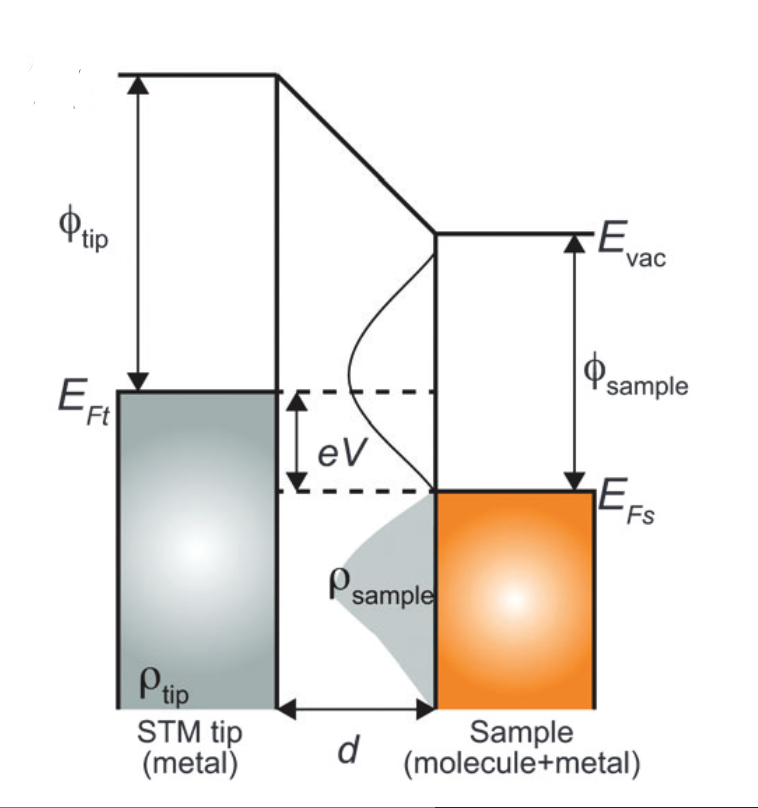
\includegraphics[width=0.4\textwidth]{graphics/Tunneling_diagram_japan.PNG}
    \caption{Energy diagram of the tunneling junction with a positive bias voltage applied. $\Phi_{tip}$ \& $\Phi_{sample}$: working functions of either tip and sample, $E_{vac}$: vacuum energy level,  $E_{ft}$ \& $E_{fs}$: Fermi Energys of the tip and sample,  $\rho_{tip}$ \& $\rho_{sample}$: density of states of tip and sample,  $eV$: potential difference caused by applying a bias Voltage $V$ (picture source: \cite{Kano}) }
    \label{fig:energy_diagram}
\end{wrapfigure}

The tunneling current, at a arbituery gridpoint, is influenced by the electronic structure of the tip and sample.
If the tip is in vicinity of the metallic substrate the fermi energies align, resulting in an equal probability of electrons tunneling from the tip to the sample and vice versa.
This consequently results in a zero net current. 
Through the introduction of a electric potential $V_{bias}$ the fermi energies of tip and sample can be shifted relative to each other (Figure \ref{fig:energy_diagram}).
If the bias voltage is positive the fermi energy of the sample is pushed down and electrons from occupied states in the tip can tunnel into the empty states of the sample.
Consequently if the bias voltage is negative electrons from the filled states of the sample tunnel into the tip.
The tunneling current is influenced by the distance $d$ between orbitals of the tip and the sample, which makes it possible to gain information about the electronic structure of the sample.
This is not really a representation of the real structure of the atoms or molecules, but the Local Density of States (LDOS) of the sample´s surface.
Utilizing this in Scanning Tunneling Spectroscopy (STS) provides additional information beyond the sample's topography.
Such as the chemical composition, bonding, the energy gap and band-bending effects \cite{cbai}.
\section{Mathematical Foundation}
\begin{wrapfigure}{r}{0.3\textwidth}
    \centering
    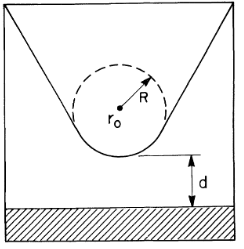
\includegraphics[width=0.3\textwidth]{graphics/fundamental_tip_sheme.PNG}
    \caption{Schematic depiction of the tip geometry \cite{PhysRevLett}}
    \label{fig:tip_scheme}
\end{wrapfigure}
To understand the tip sample interaction one must look at the quantum-mechnical Foundation behind it.
At its simplest the tip can be approximatated as spherical potential well (Figure \ref{fig:tip_scheme}). $R$ is in that case the radius of the tip located at position $\vec{r_0}$ with the distance $d$ from the surface.
First order pertubation theory gives the following expression (Eq. \ref{eq:tunneling_pert}) for the tunneling current of this system \cite{PhysRevLett}:
\begin{equation}
    I = \frac{2 \pi e}{\hbar} \sum_{\mu \nu} f(E_{\mu})[1 - f(E_{\nu}+eV_{bias})]\cdot |M_{\mu \nu}|^2 \delta(E_{\mu}- E_{\nu})
    \label{eq:tunneling_pert}
\end{equation}
\newpage

The fermi distribution $f(E)= (\exp((E-E_F)/k_b T)+1)^{-1}$ gives the ocupation probability of a fermion (electrons) with the Energy $E$ near the fermi level.
In this case it is the ocupation probability of the tip states (denoted by the subindex $\mu$) and the ocupation probability of the sample states ( denoted by the subindex $\nu$).
The tunneling matrix $M_{\mu \nu}$ is related to the derivatives of the sample wave functions $\psi_{\nu} $ at the nucleus of the apex atom \cite{tunnelmatrix}.
Because the STM Imaging is done at low temperatures and with small voltages the Equation \ref{eq:tunneling_pert} can be simplified to:
\begin{equation}
    I = \frac{2 \pi}{\hbar} e^2 V_{bias} \sum_{\mu \nu}  |M_{\mu \nu}|^2 \delta(E{\nu}-E_F) \delta(E_{\mu}- E_{F})
    \label{eq:tunneling_pert_simple}
\end{equation}
%************VERSUCHSANORDNUNG*************
\section{Experimental Setup}
\label{sec:versuchsandordnung}
The experimental work done in this thesis primarily utilized a Low-Temperature Scanning Tunneling Microscope setup.
This STM is composed of two distinct compartments, the preparation chamber (PC) the measurement chamber (MC).
The sample is inserted through a airlock into the preparation chamber.
In the whole system there is in a Ultra High Vacuum (UHV) at about 10$^{-11}$ - 10$^{-10}$ mbar, which is archieved by four individuall pumps.
The base Vacuum is achieved with the turbomolecular pump and the scroll pump through the airlock.
Additionally there is a titanium sublimation pump and a ion pump in the preparation room.

\monofig{width=\textwidth}{Experimental_Setup/STM_Picture_1_edited.pdf}{
    The experimental setup used, 
    A: cooling-chamber filled with Liquid Oxigen,
    B: measuring-chamber with spring suspended sample holder and tip,
    C: sputter-gun,
    D: metal-evaporater,
    E: molecule-evaporater,
    F: preparation-chamber with free movable sample holder arm,
    G: LEED system,
    H: Electronic used to monitor the function of the STM}{}
%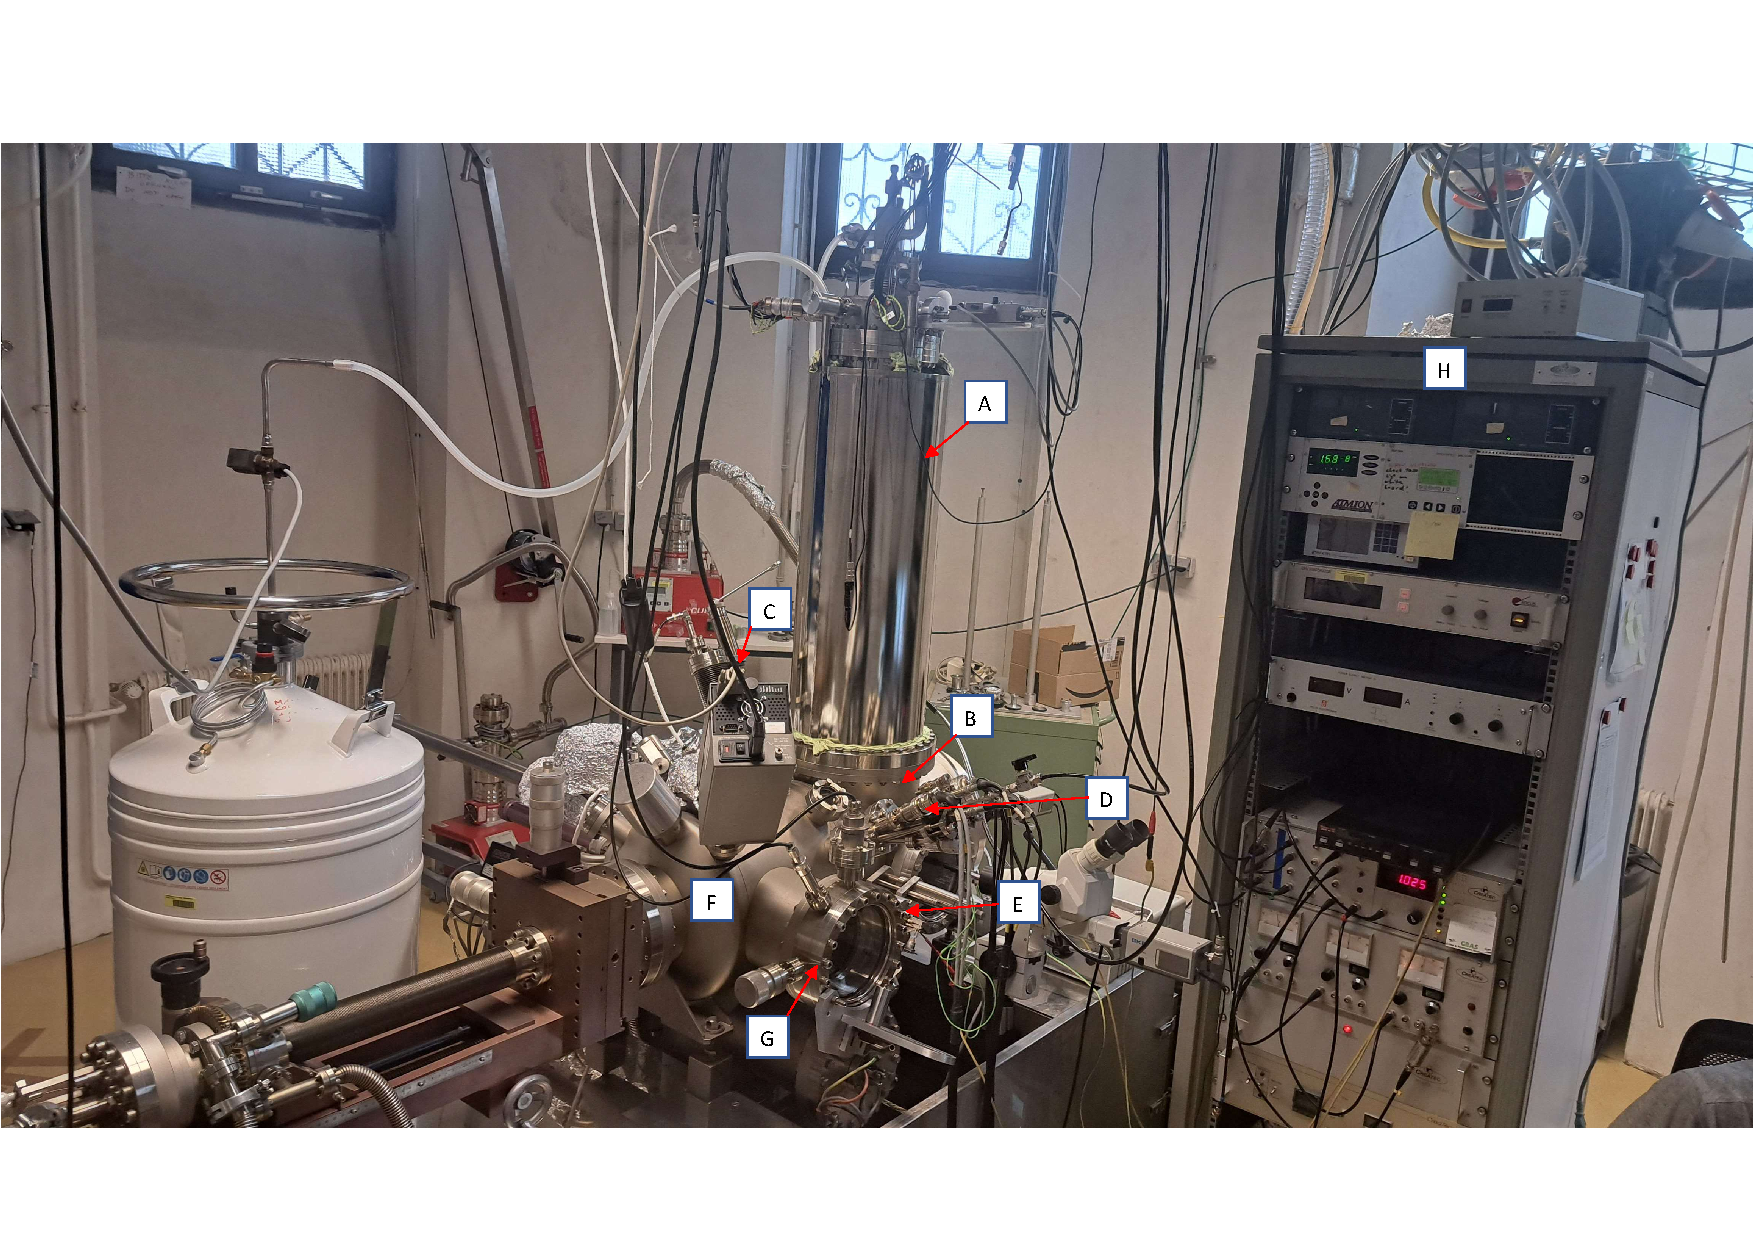
\includegraphics[width=0.9\textwidth]{Experimental_Setup/STM_Picture_1_edited.pdf}

The Probe-holder can be moved in each direction and rotated using an integrated arm in the PC.
It is also used to insert the Probe-holder into the MC.
The PC is equipped with a LEED system, which fluorescent screen can be extended 
At fixed positions in the PC there are ma
%************GERÄTELISTE***************
\section{Geräteliste}
\label{sec:geraeteliste}
\begin{table}[H]
	\centering
	\caption{
		Im Versuch verwendete Geräte und Utensilien.}
	\begin{tabularx}{1.0\textwidth}{| l | l | l | X |}
		\hline
		Gerät       & Hersteller   & Model  & technische Daten /\linebreak Unsicherheit       \\\hline
		\hline
		Laser & ThorLabs & CPS532-C2 & $\lambda$ = 532 nm; $P$ = 0.9 mW; $PER$ = 5 dB\\ \hline
		2 x Spiegel & ThorLabs & \allc & \allc \\ \hline
		4 x Doppelspalt & \allc & \allc & $b_1$ = 0.2 mm; $b_{2,3,4}$ = 0.1 mm; $a_{1,2}$ = 0.25 mm; $a_3$ = 0.5 mm; $a_4$ = 1 mm \\ \hline
		Beugungsgitter & \allc & \allc & \allc \\ \hline
		2 x Linearpolarisierungsfenster & \allc & \allc & \allc \\ \hline
		2 x Polarisatorhalterungen & ThorLabs & RSP05/M & \allc \\ \hline
		Linearpolarisierungsfolie & \allc & \allc & \allc \\ \hline
		Photodetektor & Sauter & SO 200K & \allc \\ \hline
		Linse & \allc & \allc & $f$ = 40 mm \\ \hline
		Michelson Interferometer & \allc & \allc & \allc \\ \hline
	\end{tabularx}
	\label{tab:Geraeteliste}
\end{table}
\newpage
%************VERSUCHSDURCHFÜHRUNG & MESSERGEBNISSE***********
\section{Versuchsdurchführung \& Messergebnisse}
\label{sec:versuchdurchfuehrung-messergebnisse}

\subsection{Young'scher Doppelspalt, Beugungsgitter}
\label{sec:durch:yng}
Der Aufbau des Experiments wurde gemäß Abb.\ref{fig:double_slit_aufb} realisiert.
Beim Aufbau wurde, zur Einrichtung der Spiegel, mittels einer gerasterten Platte, die Parallelität des Laserstrahls zur Montageplatte und die Umlenkwinkel von 90° eingestellt.
Das Interferenzmuster wurde auf ein kariertes Blatt Papier auf einer Wand im Abstand von $z$ = (252.6 $\pm$ 0.5) cm projiziert.
Die Muster wurden dann mit einer Smartphonekamera, auf einem Holzbrett als Bezugspunkt für konsistente Pixelauflösung, fotografiert.
Da die Kamera aber nicht parallel zur optischen Ebene ausgerichtet werden konnte (sonst wäre der Lichtstrahl bedeckt gewesen) sind die Bilder mit einer Perspektivenverzerrung behaftet.
Die Aufnahmen der Interferenzmuster für die Spalte 1-4 und das Beugungsgitter sind in Abb.\ref{fig:interf_muster} zu sehen.
\begin{figure}[h]
    \centering
    \begin{subfigure}[t]{0.4\textwidth}
        \includegraphics[width=\textwidth]{double_slit_muster1.jpeg}
        \caption{}
        \label{fig:double_slit_muster1}
    \end{subfigure}%
    \begin{subfigure}[t]{0.4\textwidth}
        \includegraphics[width=\textwidth]{double_slit_muster2.jpeg}
        \caption{}
        \label{fig:double_slit_muster2}
    \end{subfigure}
    \begin{subfigure}[t]{0.4\textwidth}
        \includegraphics[width=\textwidth]{double_slit_muster3.jpeg}
        \caption{}
        \label{fig:double_slit_muster3}
    \end{subfigure}%
    \begin{subfigure}[t]{0.4\textwidth}
        \includegraphics[width=\textwidth]{double_slit_muster4.jpeg}
        \caption{}
        \label{fig:double_slit_muster4}
    \end{subfigure}
    \begin{subfigure}[t]{0.4\textwidth}
        \includegraphics[width=\textwidth]{gitter_muster.jpeg}
        \caption{}
        \label{fig:gitter_muster}
    \end{subfigure}

    \caption{
        Aufnahmen der Interferenzmuster der 4 Doppelspalte und des Gitters.
        \ref{fig:double_slit_muster1}: Doppelspalt 1; 
        \ref{fig:double_slit_muster2}: Doppelspalt 2; 
        \ref{fig:double_slit_muster3}: Doppelspalt 3; 
        \ref{fig:double_slit_muster4}: Doppelspalt 4; 
        \ref{fig:gitter_muster}: Gitter.
    }
    \label{fig:interf_muster}
\end{figure}


\subsection{Polarisations-Analyse}

Der Aufbau des Experiments wurde gemäß Abb. \ref{fig:pol_aufbau} vollführt. 
Dabei wurde ein Spiegel um 45° zum Lot des Lichtstrahls ausgerichtet, um diesen um 90° umzulenken.
Es wurde,mittels einer gerasterten Platte, auf die Parallelität des Strahl überprüft.
Hierbei ist entscheidend, dass der gesamte Strahlengang, sowohl horizontal (parallel zu den Befestigungslöcher) als auch vertikal (parallel zum Befestigungstisch) ausgerichtet wird.
Es wurde darauf geachtet, dass der Strahl möglichst Zentral den Intensitätssensor trifft.
Anschließend wurde ein Rohr vor das Luxmeter gestellt, um den Sensor von jeglicher Hintergrundstrahlung abzuschirmen.
Es wurde angenommen, dass der Laser linear polarisiert ist, was die Bestimmung der Vorzugsrichtung der Polarisation erfordert.
Dies wurde getan um die Grundintensität nach dem ersten Polarisator maximal zu halten.
Der Winkel des Polarisators wurde bei dieser Position aufgenommen ($\beta_{1,0}$ = (13 $\pm$ 2)°)
Natürlich gibt es hierbei trotzdem eine Reduzierung der ausgehenden Lichtintensität des Lasers, ausgelöst durch die Interaktion der elektromagnetischen Welle mit den Kristallgitter des Polarisators sowie der Unschärfe in der Polarisationsrichtung des Lasers.
Zuletzt wurde der zweite Polarisator, nach dem ersten, in den Strahlengang gebracht und wieder die Position der maximalen Lichtintensität gesucht ($\beta_{2,0}$= (275 $\pm$ 2)°).
Dieser wurde anschließend in 10° Schritten gedreht und dabei die Lichtintensität aufgezeichnet.


\begin{table}[H]
    \label{tab:pol}
    \centering
    \captionof{table}{
        Experimentell bestimmte Werte. Die Unsicherheit im Winkel wurde mit 2° angenommen und die Unsicherheit der Intensität laut dem Datenblatt \cite{LUX}  berechnet.
        $\beta_1$: Winkel des ersten Polarisators
        $\beta_2$: Winkel des zweiten Polarisators,
        $I$: gemessene Lichtintensität}
    \begin{tabular}{ccc} \hline
    $\beta_1$ / ° & $\beta_2$ / ° & $I$ / Lux \\\hline \hline
    $13$&$275$&$597$\\ \hline
    $20$&$275$&$577$\\ \hline
    $30$&$275$&$503$\\ \hline
    $40$&$275$&$392$\\ \hline
    $50$&$275$&$266$\\ \hline
    $60$&$275$&$164$\\ \hline
    $70$&$275$&$83$\\ \hline
    $80$&$275$&$31$\\ \hline
    $90$&$275$&$9$\\ \hline
    $100$&$275$&$0$\\ \hline
    $110$&$275$& $1$\\ \hline
    $120$&$275$&$13$\\ \hline
    $130$&$275$&$44$\\ \hline
    $140$&$275$&$102$\\ \hline
    $150$&$275$&$192$\\ \hline
    $160$&$275$&$298$\\ \hline
    $170$&$275$&$412$\\ \hline
    $180$&$275$&$504$\\ \hline
    $190$&$275$&$550$\\ \hline
    $195$&$275$&$554$\\ \hline
    \end{tabular}
\end{table}
Im letzten Teil der Polarisations-Analyse wurde der Einfluss eines weiteren Polarisators, welcher zwischen den beiden ursprünglichen Polarisatoren gebracht,untersucht.
Zunächst werden die Filter so eingestellt, dass ihre Polarisationsebenen 90° zu einander stehen (siehe Abb \ref{fig:polmin}).
\duofigcom{pol_2polMin2.jpg}{fig:polmin1}{pol_3polMin1.jpg}{fig:polmin2}{(a) Lichtintensität bei 90° Differenzwinkel. (b) Hier ist die Polarisationsebene des ersten Polarisators zu sehen}{fig:polmin}
Wenn man nun den Filter um 45° dreht, ist ein Intensitätsmaximum zu sehen, da das Licht nun nicht mehr einen Differenzwinkel von 90° zum zweiten Polarisator hat.
\duofigcom{pol_3polMax2.jpg}{fig:polmin1}{pol_3polMax1.jpg}{fig:polmin2}{(a) \& (b) Intensitätsmaximum bei 45 ° Differnezwinkel zu beiden Polarisatoren }{fig:polmin}

\subsection{Michelson-Interferometer}
Um das Michelson Interferometer in Betrieb zu nehmen, muss der Strahlengang eingestellt werden.
Dazu wurde ,wie zuletzt, dieser sowohl parallel zum Tisch als auch parallel zu den Fixierungslöchern eingestellt.
Anschließend wurden die beiden Spiegel (siehe Abb. \ref{fig:michelson_inter}) so eingestellt, dass die zwei reflektierten Strahlen sich am Abbildungsschirm überlagern.
\subsubsection{konzentrisches Interferenzmuster}
Bringt man nun die Linse (siehe Abb \ref{fig:michelson_inter} ,f= 40 mm) vor den Eingang des Interferometers bildet sich ein konzentrisches Interferenzmuster am Abbildungsschirm (siehe Abb. \ref{fig:inter_ges}).
Dabei ist bemerkbar, dass das Zentrum der Interferenzringe mit der Winkeleinstellung des Spiegels $D$ (siehe Abb. \ref{fig:michelson_inter}) verschoben werden kann. 
Hingegen führt die Änderung des Abstandes des Spiegels $C$ ein Verschieben der Interferenzmaxima bzw. -Minima in der Abbildungsebene.
In Abb.\ref{fig:inter_ges} sind zwei konzentrische Interferenzmuster mit unterschiedlichen Einstellungen der Spiegel $D$ und $C$ zu sehen.
\duofigcom{konz_inter_3.jpeg}{fig:inter_klein}{konz_inter_gross.jpeg}{fig:inter_gross}{(a) konzentrisches Interferenzmuster bei größerer Differenz der Armlängen (b) konzentrisches Interferenzmuster bei annäherend gleichen Armlängen}{fig:inter_ges}

Zur Verifikation des komplementären Musters an beiden Ausgängen des Interferometers wurde ein Loch in ein Blatt Papier gestanzt und dieses dann zwischen Linse und Interferometer genau am Brennpunkt der Linse gehalten.
Die beiden Muster sind in Abb.\ref{fig:konz_inter_2} zu sehen.

\begin{figure}[H]
    \centering
    \begin{subfigure}[t]{0.45\textwidth}
        \includegraphics[width=\textwidth]{konz_inter_2.jpeg}
        \caption{}
        \label{fig:konz_inter_2_schirm}
    \end{subfigure}
    \begin{subfigure}[t]{0.45\textwidth}
        \includegraphics[width=\textwidth]{konz_inter_2_komp.jpeg}
        \caption{}
        \label{fig:konz_inter_2_komp}
    \end{subfigure}

    \caption{
        Aufnahmen der Interferenzmuster am Schirm und im Laserarm.
        \ref{fig:konz_inter_2_schirm}: Muster am Schirm; 
        \ref{fig:konz_inter_2_komp}: komplementäres Muster im Laserarm.
    }
    \label{fig:konz_inter_2}
\end{figure}



Um die Wellenlänge des Lasers zu bestimmen wurde das Interferenzzentrum aus der Bildebene gebracht und die Position des Spiegels $C$ variert.
Dabei wurden 2 Messdurchgänge gemacht in denen die Anzahl der Interferenzmaxima-Übergänge $N$ abgezählt und die relative Längenänderung $\Delta x$ aufgezeichnet wurde.
Danach wurde der Spiegel $C$, zur Bestimmung dessen Position bei absolut gleicher Armlängen, in die Position gebracht in der das zentrale Interferenzmaxima am weitesten ausgedehnt wurde (siehe Vgl. Abb.\ref{fig:fig:inter_ges}), und die Position an der Mikrometerschraube $x_0$ abgelesen.
Die Messergebnisse sind in Tab.\ref{tab:inter_konz} aufgelistet.
\begin{table}[H]
    \centering
    \captionof{table}{
        Messungen für die Wellenlängenbestimmung und der Position absolut gleich langer Interferometerarme.
        \textbf{Nr.}: Messnummer; 
        \textbf{Bez.}: Messbezeichnung; 
        $N$: Anzahl der Interferenzmaxima-Übergänge mit Unsicherheit aus grober Abschätzung wie oft verzählt wurde; 
        $\Delta x$: relative Längenänderung an der Mikrometerschraube des Spiegels C mit Unsicherheit der Mikrometerschraube; 
        $x_0$: Position der Mikrometerschraube bei absolut gleichen Weglängen mit abgeschätzter Unsicherheit resultierend daraus wie genau die maximale Ausdehnung des zentralen Interferenzmaxima erkannt werden konnte.
    }
    \begin{tabular}{|c|cc|cc|} \hline
        Nr. & Bez.          & Messwert          & Bez.                  & Messwert \\\hline \hline
        1   & $N$ / 1       & 22 $\pm$ 1        & $\Delta x$ / $\mu$m   & 35 $\pm$ 1 \\ \hline
        2   & $N$ / 1       & 50 $\pm$ 2        & $\Delta x$ / $\mu$m   & 70 $\pm$ 1 \\ \hline \hline
        3   & $x_0$ / mm    & 12.5 $\pm$ 0.1    &                       &  \\ \hline
    \end{tabular}
    \label{tab:inter_konz}
\end{table}


\subsubsection{paralleles Interfernezmuster}
Als nächstes wurde die Linse zwischen Ausgang und dem Abbildungsschirm platziert (Abb. \ref{fig:parallel_danach}). 
Es wurde leider fälschlicherweise die gleiche Linse benutzt, obwohl eine Linse mit einer Brennweite von 16 mm benutzt werden sollte.
Das einbringen der Linse nach dem Ausgang führt nun zu einem parallelen Streifenmuster (Abb. \ref{fig:parallel_muster}).
\duofigcom{michl_paralell_muster.jpg}{fig:parallel_muster}{michl_paralell_linse_danach.jpg}{fig:parallel_danach}{(a) Aufgenommenes paralleles Interferenzmuster, (b) Position der Linse bei der Aufnahme}{fig:parallel_ges}
\subsubsection{Polarisation}
Zuletzt wurde ein Polarisator vor den Eingang des Interferometers gebracht. 
Die Durchlassrichtung des Polarisators wurde mit einem weiteren Polarisator bestimmt, indem dieser solange gedreht wurde bis kein Licht mehr transmittiert wurde.
Dies entspricht einem Winkelversatz von 90° und kann genutzt werden um den Polarisator um 45 grad zum Tisch auszurichten.
Nun wurden die beiden Folienpolarisatoren in die Arme eingebracht und verschiedene Kombinationen der relativen Drehung ausprobiert.
\begin{figure}[h]
    \centering
    \begin{subfigure}[t]{0.4\textwidth}
        \includegraphics[width=\textwidth]{michelson_pol_00_aufb.jpeg}
        \caption{}
        \label{fig:michelson_pol_00_aufb}
    \end{subfigure}%
    \begin{subfigure}[t]{0.4\textwidth}
        \includegraphics[width=\textwidth]{michelson_pol_00_schirm.jpeg}
        \caption{}
        \label{fig:michelson_pol_00_schirm}
    \end{subfigure}
    \begin{subfigure}[t]{0.4\textwidth}
        \includegraphics[width=\textwidth]{michelson_pol_90_aufb.jpeg}
        \caption{}
        \label{fig:michelson_pol_90_aufb}
    \end{subfigure}%
    \begin{subfigure}[t]{0.4\textwidth}
        \includegraphics[width=\textwidth]{michelson_pol_90_schirm.jpeg}
        \caption{}
        \label{fig:michelson_pol_90_schirm}
    \end{subfigure}

    \caption{
        Aufnahmen der Interferenzmuster am Michelson Interferometer bei Polarisierten Teilstrahlen.
        Aufbau \ref{fig:michelson_pol_00_aufb} und Muster am Schirm \ref{fig:michelson_pol_00_schirm} bei zwei horizontal ausgerichteten Polarisatoren; 
        Aufbau \ref{fig:michelson_pol_90_aufb} und Muster am Schirm \ref{fig:michelson_pol_90_schirm} bei einem horizontal  und einem vertikal ausgerichteten Polarisator.
    }
    \label{fig:michelson_pol}
\end{figure}


\newpage
%************AUSWERTUNG****************
\section{Auswertung}
\label{sec:auswertung}
Die Auswertung wird mit der Skriptingsprache \verb|Python| \cite{PYTHON} erstellt.
In der gesamten Auswertung werden die Python Libraries, \verb|numpy| \cite{harris2020array}, \verb|pandas| \cite{reback2020pandas}, \verb|scipy| \cite{2020SciPy-NMeth} und \verb|matplotlib| \cite{Hunter:2007}, für statistische Rechenoperationen, das Einlesen und Verarbeiten von Daten sowie das Erstellen von Plots verwendet.
Genaue Funktionsnamen, die zur Berechnung von Messgrößen oder Fit-Parametern verwendet werden, sind in der weiteren Auswertung angegeben.
Des weiteren wird die Library \verb|uncertainties| \cite{UN} für jegliche Unsicherheitsfortpflanzungen (wenn nicht anders angegeben) benutzt, da diese auf dem Prinzip der Größtunsicherheitsmethode Gl. \ref{equ:groestunsicherheit} basiert.


\subsection{Young'scher Doppelspalt, Beugungsgitter}
Da die Aufnahmen aus Abb.\ref{fig:interf_muster} der Beugungsmuster eine Perspektivenverzerrung aufweisen wird diese vorerst mit der Software FIJI (Plugin "Transform -> Interactive Perspective") korrigiert.
Dabei orientiert man sich an einem Äquidistanten Gitter, welches über das Bild gelegt wird und korrigiert durch verzerren von 4 Punkten am Bild.
Die korrigierten Bilder mit vergleichsgitter sind in Abb.\ref{fig:interf_muster_corr_grid} zu sehen.
\begin{figure}[h]
    \centering
    \begin{subfigure}[t]{0.4\textwidth}
        \includegraphics[width=\textwidth]{double_slit_muster1_corr_grid.jpg}
        \caption{}
        \label{fig:double_slit_muster1_corr_grid}
    \end{subfigure}%
    \begin{subfigure}[t]{0.4\textwidth}
        \includegraphics[width=\textwidth]{double_slit_muster2_corr_grid.jpg}
        \caption{}
        \label{fig:double_slit_muster2_corr_grid}
    \end{subfigure}
    \begin{subfigure}[t]{0.4\textwidth}
        \includegraphics[width=\textwidth]{double_slit_muster3_corr_grid.jpg}
        \caption{}
        \label{fig:double_slit_muster3_corr_grid}
    \end{subfigure}%
    \begin{subfigure}[t]{0.4\textwidth}
        \includegraphics[width=\textwidth]{double_slit_muster4_corr_grid.jpg}
        \caption{}
        \label{fig:double_slit_muster4_corr_grid}
    \end{subfigure}
    \begin{subfigure}[t]{0.4\textwidth}
        \includegraphics[width=\textwidth]{gitter_muster_corr_grid.jpg}
        \caption{}
        \label{fig:gitter_muster_corr_grid}
    \end{subfigure}

    \caption{
        Perspektivenkorrigierte Aufnahmen der Interferenzmuster mit eingezeichnetem Vergleichsgitter.
        \ref{fig:double_slit_muster1_corr_grid}: Doppelspalt 1; 
        \ref{fig:double_slit_muster2_corr_grid}: Doppelspalt 2; 
        \ref{fig:double_slit_muster3_corr_grid}: Doppelspalt 3; 
        \ref{fig:double_slit_muster4_corr_grid}: Doppelspalt 4; 
        \ref{fig:gitter_muster_corr_grid}: Gitter.
    }
    \label{fig:interf_muster_corr_grid}
\end{figure}
An den korrigierten Aufnahmen werden dann mit der PIL(Python Image Library) die Pixel in ihren RGB CHannel Werten gefilter, so dass nur Pixel mit Wertigkeit größer als 160 überbleiben.
Dies ist nötig um ein gutes Interferenzsignal zu erhalten.
Danach wird aus jedem Bild nur der Bereich ausgeschnitten in dem das Interferenzmuster zu sehen ist.
Die Ausgeschnittenen Bereiche sind in Abb.\ref{fig:yng_cutouts} zu sehen.
\monofig{width=0.7\textwidth}{yng_cutouts.pdf}{
    Ausschnitte der RGB gefilterten Aufnahmen.
    Von Oben nach unten für die Doppelspalte 1 bis 4 und für das Beugungsgitter.
}{fig:yng_cutouts}
Um die eindimensionalen Interferenzmuster zu erhalten werden die Ausschnitte aus Abb.\ref{fig:yng_cutouts} in Grauwert Bilder umgewandelt, ihre Pixelwerte über alle Reihen summiert und dann auf den Maximalwert normiert.
Um die räumliche Auflösung des Interferenzmusters zu erhalten wird an den Bildern abgezählt wie viele Kästchen in horizontaler Richtung des Referenzgitters am Bild sind, da die Breite dieser Kästchen mit $d_K$ = 5 mm genau bekannt ist.
Die Interferenzmuster der Doppelspalte werden dann nach Gl.\ref{eq:gru:Int-mult}, Gl.\ref{eq:gru:Int} und Gl.\ref{eq:gru:Beug} mit Spaltparametern $a_i$ und $b_i$ gefittet um die Wellenlänge des Lasers zu erhalten.
Das Interferenzmuster des Gitters Wird nach Gl.\ref{eq:ausw:gitter} mit $\lambda$ = 532 nm, Schirmabstand $z$ aus Kap.\ref{sec:durch:yng} und einer geschätzten beleuchteten Spaltanzahl $N$ = 7 gefittet um den Spaltabstand $b$ zu erhalten.
\begin{equation}
    I_{G,th}(x) = \frac{sin^2\left(N \frac{\pi b x}{\lambda z}\right)}{N^2 sin^2\left(\frac{\pi b x}{\lambda z}\right)}
    \label{eq:ausw:gitter}
\end{equation}
Die erhaltenen Interferenzmuster und Fitfunktionen sind in Abb.\ref{fig:yng_fits} zu sehen.
Die erhaltenen Fitparameter sind in Tab.\ref{tab:yng-Werte} gelistet
\monofig{width=0.7\textwidth}{yng_fits.pdf}{
    Interferenzmuster und deren Fitfunktionen.
    Von Oben nach unten für die Doppelspalte 1 bis 4 und für das Beugungsgitter.
}{fig:yng_fits}
\begin{table}[H]
    \centering
    \caption{
        Ermittelte Fitparameter der Interferenzmuster
    }
    \begin{tabular}{cc} \hline
        Bezeichnung & Wert \\ \hline
        $\lambda_{S1}$  & (552 $\pm$ 13) nm \\ \hline
        $\lambda_{S2}$  & (536 $\pm$ 6 ) nm\\ \hline
        $\lambda_{S3}$  & (528 $\pm$ 3 ) nm\\ \hline
        $\lambda_{S4}$  & (524 $\pm$ 1 ) nm\\ \hline
        $b$  & (125.73 $\pm$ 0.03) $\mu$m \\ \hline
    \end{tabular}
    \label{tab:yng-Werte}
\end{table}

\subsection{Gesetz von Malus}
Die bestimmten Winkel $\beta_1$ und $\beta_2$ bei der maximalen Lichtintensität entsprechen effiktiv einen Winkelversatz der Polarisationsebenen von 0°.
Der Differenzwinkel $\alpha$ ergibt sich zu:
\begin{equation}
    \alpha_i = |\beta_{1,i}- \beta_{1,0}|
\end{equation}
Trägt man nun die Intensität gegen den Winkel $\alpha$ auf kommt das Gesetz von Malus zu Vorschein. Dabei ist sichtbar das einen trigometrischen Verlauf hat.
\monofig{width=0.8\textwidth}{Polar_errobars.png}{Gegenüberstellung der aufgenommenen Datenpunkte zu theoretischen Kurve}{fig:malus}
In Abbildung \ref{fig:malus} ist sichtbar , dass es eine relativ große Diskrepanz zwischen Theorie und Messwert gibt. 
Dies ist vermutlich auf die Polarisation des Lasers zurückzuführen.
Bei der Durchführung des Experiments wurde fälschlicherweise angenommen, dass die Wahl des zu drehenden Polarisators keinen Unterschied macht und nur der Differenzwinkel wichtig ist.
Wird unpolarisiertes Licht als Quelle benutzt, ist dies auch der Fall, doch im Falle des Lasers wird polarisiertes Licht emittiert.
Der Laser ist vermutlich leicht elliptisch polarisiert und hat eine Richtung,in dem das elektrische Feld eine höhere Amplitude hat.
Verdreht man nun den ersten Polarisator, kommt es zu einer Reduktion der Intensität durch die sich verändernde Amplitude des E-Felds und zusätzlich durch den Differenzwinkel zum zweiten Polarisator.
Das bedeutet, dass die Intensität $I_0$ auch von $\alpha$ abhängt.
Da die Polarisatoren früher so eingestellt worden sind, dass die Lichtintensität maximal ist, kann angenommen werden, dass hier die maximale Auslenkung des E-felds liegt.
Die elliptische Auslenkung des E-Feldes kann mittels einer Kurve modeliert werden $\vec{E} \propto  (a \cdot \cos(\alpha), b \cdot \sin(\alpha) )$.
Der Quadrat des Abstandes der Kurve zum Mittelpunkt sollte proportional zur Intensität sein ($I_0(\alpha) \propto |\vec{E}|^2$).
\begin{equation}
    I_0(\alpha) = I_0 \cdot ((a\cos(\alpha))^2 + (b\sin(\alpha))^2)
\end{equation}
Wendet man nun die Korrektur auf die Ausgangsgleichung \ref{eq:malus} an, erhält man:
\begin{equation}
    I(\alpha) = I_0 \cdot ((a\cos(\alpha))^2 + (b\sin(\alpha))^2)\cdot \cos^2(\alpha)
\end{equation}
Fittet man nun die Parameter $a$ und $b$ kann man die Polarisierung ausgleichen.
Zusätzlich wurde aus dem Datenblatt des Lasers erhoben,dass die PER (Polarization extinction ratio ) 5 dB ist.
Nun kann mittels Gl. \ref{eq:per}  (siehe \cite{PER}) das Verhätniss der Leistung der elektromagnetischen Welle in den beiden Halbachsen der Ellipse gefunden werden.
\begin{equation}
    \frac{a}{b} = \frac{P_{max}}{P_{min}} = 10^{\frac{\text{PER}}{10}} = 3.162
    \label{eq:per}
\end{equation}

Es wurde nun auch die Korrektur mittels den bekannten Polarisationskonstanten  des Lasers durchgeführt.
Dabei wird $a =1$ und $b = 1/3.162$ angenommen, da wir den ersten Polaristator auf die große Halbachse der Polarisationellipse des Lasers ausgerichtet haben.
Das modifizierte Gesetz von Malus lautet in diesem Fall :
\begin{equation}
    I(\alpha) = I_0  \biggl( \cos^2(\alpha) + \biggl( \frac{\sin(\alpha)}{3.162} \biggr)^2 \biggr) \cdot \cos^2(\alpha)
\end{equation}
\monofig{width=0.8\textwidth}{Polar_korrektur3.png}{Korrektur der ursprünglichen Gleichung durch Fit und den erhobenen Parameter des Lasers}{fig:korr}
Die Koeffizienten a und b ergeben sich zu: 
\begin{align}
    a &= 0.97 \\
    b &= 0.47 \\
    \frac{a}{b} &= 2.1
    \label{eq:ab}
\end{align}

\subsection{Michelson-Interferometer}
Mit den Messdaten aus Tab.\ref{tab:inter_konz} werden nach Gl.\ref{eq:ausw:hebel} die wirklichen Längenänderungen des Interferometerarms $\Delta x'$ berechnet, da am Spiegel C ein Hebel angebaut ist.
\begin{equation}
    \Delta x' = \frac{\Delta x}{5.3}
    \label{eq:ausw:hebel} 
\end{equation}
Weiters wird dann über Gl.\ref{eq:ausw:lamb} die Wellenlänge des Lasers bestimmt.
\begin{equation}
    \lambda = \frac{2\Delta x'}{N}
    \label{eq:ausw:lamb} 
\end{equation}
Die berechneten Wellenlängen mit Unsicherheit sind in Tab.\ref{tab:ausw:michelson} gelistet
\begin{table}[H]
    \centering
    \caption{
        Ermittelte Wellenlängen durch Michelson Interferometer.
    }
    \begin{tabular}{cc} \hline
        Bezeichnung & Wert \\ \hline
        $\lambda_{1}$  & (600 $\pm$ 50) nm \\ \hline
        $\lambda_{2}$  & (528 $\pm$ 30 ) nm\\ \hline
    \end{tabular}
    \label{tab:ausw:michelson}
\end{table}
%************DISKUSSION***************
\chapter{Discussion}
\label{sec:Discussion}



\printbibliography
\end{document}